\documentclass[en,hazy,blue,screen,14pt]{elegantnote}
\usepackage[T1]{fontenc}
\usepackage[latin9]{inputenc}
% \usepackage[USenglish]{babel}
\usepackage{babel}
% TODO: interesting bug about the font of proof env
\usepackage{float}
\usepackage{textcomp}
\usepackage{amsmath,amsfonts,amssymb}
\usepackage{amsthm}
\usepackage{graphicx}
\usepackage[ruled,vlined]{algorithm2e}
\PassOptionsToPackage{normalem}{ulem}
\usepackage{ulem}
\usepackage{mathtools}
\usepackage{url}
\usepackage{hyperref}

\DeclarePairedDelimiter{\ceil}{\lceil}{\rceil}
\newcommand\tab[1][1cm]{\hspace*{#1}}
\newenvironment{claim}[1]{\par\noindent\underline{Claim:}\space#1}{}
\newenvironment{claimproof}[1]{\par\noindent\underline{Proof:}\space#1}{\hfill $\blacksquare$}

\title{Class Notes\\CIS 502 Analysis of Algorithm\\4-Greedy Algorithm}
\author{Da Kuang}
\institute{University of Pennsylvania}
% \version{1.00}
\date{}

\begin{document}

\maketitle
\newpage
% % 
\section{Optimization Problem}
\begin{definition}
\textbf{Optimization Problem:} Minimize or maximize some function subject to 
some constrains.
\end{definition}

Now we start with a special class of optimization problem:

\begin{itemize}
 \item Given a set of elements, pick a subset.
 \item Constrains tell you which subsets are allowed.
 \item Any allowed subset is a feasible solution.
 \item Objective function assigns a value to every feasible solution.
 \item Goal is to find the feasible solution with greatest/ least value.
\end{itemize}
ddd


\subsection{Minimum Spanning Tree Problem}
Minimum spanning tree problem is an example of optimization problem.
\paragraph{Input:} Connected, undirected graph $G \in (V,~E)$ together with a 
weight function $w: E \rightarrow \mathbb{R}^+$.

\begin{definition}
 The \textbf{feasible solution} is a set of edges forming an acyclic connected 
graph on all vertices.
\end{definition}

\begin{definition}
 The \textbf{cost} of a solution is the sum of the weights of the edges in the 
solution.
\end{definition}

The are problems for which the optimal solution can be pick by choosing one 
element at a time.

\begin{definition}
The \textbf{greedy algorithm} builds up solution as by taking the next element 
to be one of the optimal cost value that can be added feasibly.
\end{definition}

Most of the time Greedy algorithm itself is simple but it is difficult to prove 
correctness.



\section{Activity Selection Problem}
\begin{itemize}
 \item \textbf{Input:} $n$ activities $a_1, \cdots, a_n$, where $a_i$ starts at 
time $x_i$ and ends at time $y_i$.
\item \textbf{Feasible Solution:} Any subset of these activities such that no 
two activities in the subset overlap. 
\item \textbf{Objective Function:} Maximize the number of activities we 
schedule.
\end{itemize}

\subsection{Some Attempts}
Criterions to be greedy on:
\begin{itemize}
	\item Pick the activities with shortest duration. 
	
	It dose not work. The counter example is as follows:
    \begin{figure}[H]
    \centering
    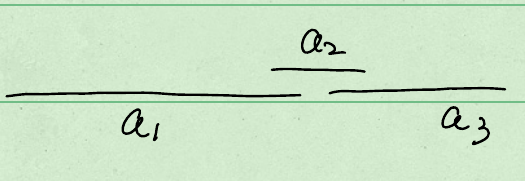
\includegraphics[width=0.3\textwidth]{1st-attempt.png}
    \end{figure}
	\item Pick the activities what finish first.\\
        Sort the activities by finish time and then renumber them so that $f_1 
\le f_2 \cdots \le f_n$
\end{itemize}
\subsection{Proposed Greedy Algorithm}
Given a set of activities, 
\begin{itemize}
	\item Pick the earliest finishing activities that remain.
	\item Remove all activities that conflict with the chosen activity.
	\item Repeat.
\end{itemize}

To prove the correctness, we start by arguing that the algorithm 
is not wrong on its first choice.

\begin{claim}
	\textbf{Greedy Choice Property:} First choice made by greedy algorithm is 
not wrong.
\end{claim}
To be more specific, in activities selection problem, if greedy algorithm 
choose an activity at first, then there is an optimal feasible solution that 
contain $a_1$.

\begin{claimproof}
	Suppose for contradiction that no optimal feasible solution uses $a_1$. 
Let $O$ be the subset of activities in some optimal solution. We can order the 
activities in $O$ by finish time.

    Let $a_{i1}, a_{i2}, \cdots, a_{ik}$ be the activities in $O$ so ordered. 
We can make an \textbf{exchange argument} as the following plot. Throw out 
$a_i$ from $O$ and include $a_1$ in instead to get a new set of activities 
$O'$. 

    There are some properties about $O'$.
    \begin{itemize}
        \item $|O'| = |O|$
        \item $O'$ is feasible.
        \item $O'$ is also optimal and contains $a_1$. 
$\Rightarrow\mskip-\thinmuskip\Leftarrow$
    \end{itemize}

    \begin{figure}[H]
    \centering
    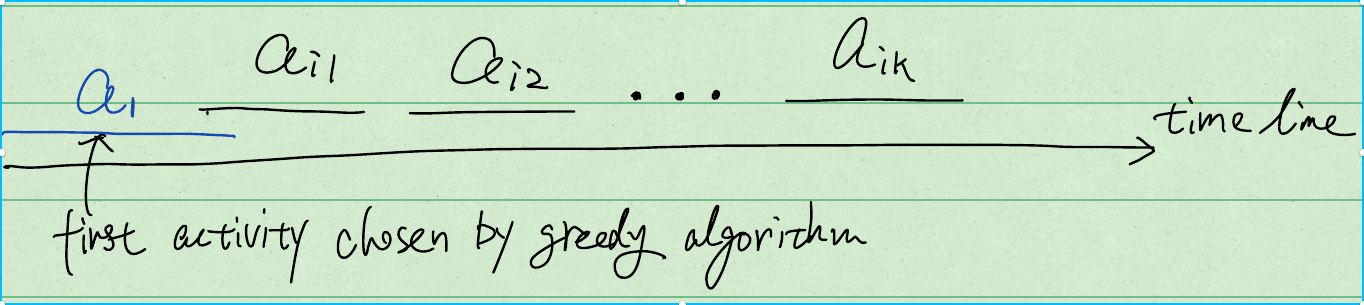
\includegraphics[width=0.5\textwidth]{exchange-selection-1.png}
    \end{figure}
\end{claimproof}

There is a way to construct an optimal solution starting with $a_1$. This 
optimal solution should certainly exclude activities that conflict with $a_1$. 
Recursively need to solve a smaller problem consisting of activities that do 
not conflict with $a_1$. In particular, the smaller problem is finding the 
optimal subset of activities out of the remaining activities.

\begin{claim}
    \textbf{Optimal Substructure Property}
	In the set of activities, we need to pick an optimal feasible 
subset activities.
\end{claim}
\begin{claimproof}{}
\begin{itemize}
	\item $A$: Original set of activities
	\item $A'$: Set of activities that remain after throwing out $a_1$ and 
its conflicting activities.
\end{itemize}
    Any solution to $A'$ that gives value $k$ can be extended to a solution to 
$A$ of value $(k+1)$ by adding $a_1$. So need optimal solution to $A'$
\end{claimproof}

In general. Optimal Substructure Property inductively assumes that greedy 
solves problem with fewer than $n$ activities optimally.

Greedy Choice Property and Optimal Substructure Property imply that greedy 
solve $n$-activity problem optimally.

\subsubsection{Time}
We sort the activities by finish time take $O(n\log n)$. Then the rest of steps 
can be done in linear or constant time.


\section{Linear Algebra}
\begin{definition}
	$V$ is a \textbf{vector space over $\mathbb{R}$} if
	\begin{itemize}
		\item For $v_1, ~v_2 \in V$, $v_1 + v_2 \in V$.
		\item For any $\alpha \in \mathbb{R}, ~v \in V$, $\alpha v \in V$.
	\end{itemize}
\end{definition}

\begin{definition}
    Given a finite set of vectors, $v_1, v_2, \cdots, v_k$, then \textbf{span} 
$S$ is as 
    follows
    \[S(v_1, v_2, \cdots, v_k) = \{v: v = \alpha_1 v_1 + \alpha_2 v_2 + \cdots 
    +\alpha_k v_k, ~\alpha_i \in \mathbb{R}\}\]
\end{definition}
$S(v_1, v_2, \cdots, v_k)$ is a vector space.

\begin{definition}
	$\alpha_1 v_1 + \alpha_2 v_2 + \cdots +\alpha_k v_k$ is a \textbf{linear 
combination} of vectors. 
\end{definition}

\begin{definition}
    The set of vector $v_1, \cdots, v_k$ is called \textbf{linear dependent} if 
there exist some coefficient $\alpha_1, \cdots, \alpha_k$ not all $0$, so that 
$\sum \alpha_i v_i = 0$
\end{definition}

\begin{definition}
	A set of vector is said to be \textbf{linearly independent} if it is not 
linearly dependent.
\end{definition}

\begin{definition}
	If $v_1, \cdots, v_k$ are linearly independent and their span in $V$, then 
$v_1, \cdots, v_k$ form a \textbf{basis} of $V$.
\end{definition}

\begin{definition}
	If $v_1, \cdots, v_k$ is a basis for $v$ and $u_1, \cdots, u_m$ is another 
basis. Then $m = k$.
\end{definition}

\begin{proof}
	Suppose for contradiction that $m > k$. Since $v_i$'s from a basis,
	\begin{align*}
		u_1 &= \alpha_{11} v_1 + \cdots + \alpha_{1k}v_k\\
		u_2 &= \alpha_{21} v_1 + \cdots + \alpha_{2k}v_k\\
            &\vdots\\
        u_m &= \alpha_{m1} v_1 + \cdots + \alpha_{mk}v_k\\
	\end{align*}
Will prove $(u_1, \cdots, u_m)$ is linearly dependent. Need to show
$\sum x_i u_i = 0$ for some $(x_1, \cdots, x_m)$ not all zero.
\begin{align*}
	&x_1 u_1 + x_2 u_2 + \cdots + x_m u_m = 0\\
	\intertext{substitue $u_i$ with $v_i$'s,}
	&(x_1 \alpha_{11} + x_2 \alpha_{21} + \cdots + x_m \alpha_{m1}) v_1\\
	+~& \cdots\\
	+~&(x_1 \alpha_{1k} + x_2 \alpha_{2k} + \cdots + x_m \alpha_{mk}) v_k = 0
\end{align*}
All the coefficients above should be 0. There are $k$ coeficientes, $m$ 
equations and we assume $m > k$. Therefore, there are infinite possible 
combinations of $x_i$'s. Therefore, there must be a solution which is not 
all zeros. Because if there is not such solution, then there should be only one 
solution which is all zeros.
\end{proof}




\section{Maximum Total Weight Problem}
Suppose you are Google and you assign a vector to each possible document. When
a user searches for a term, you want to collect some vectors that are indicative of that search term. You also want to be diverse, e.g., if a user searches for "jaguar" you want to return some documents with cars and others with the animal. We could model this by returning vectors that are linearly independent.

\begin{itemize}
	\item \textbf{Inputs:} vectors $(v_1, v_2, \cdots, v_n)$ with weights 
$(w_1, w_2, \cdots, w_n)$.
    \item \textbf{Goal:} Find a basis for the space spanned by $(v_1, v_2, \cdots, 
v_n)$ of maximum total weights.
\end{itemize}
\paragraph{Note.} A single vector is linear independent to any other vector if 
it is a zero vector.

\subsection{Greedy Algorithm}
\begin{itemize}
	\item Sort vectors and renaming them by descending order of weights.
	\item $S$ is an empty set of vectors initially.
	\item For each vectors $v_i$ in this order, if $S \cup \{v_i\}$ is linearly 
independent and $v_i$ is an non-zero vector, then $S = S \cup \{v_i\}$.
\end{itemize}

\subsection{Correctness}
\begin{theorem}
	\textbf{(Exchange Property)} Suppose A and B are finite subset of linearly independent vectors in $ \mathbb{R}^d $, and suppose $ |A| < |B| $. $\exists b \in B$, such that $ A \cup \{b\} $ in linearly independent.
\end{theorem}

\begin{proof}
	Indeed, there must be a vector in $ B $ that lies outside the space spanned by $ A $ because of the dimensions of space $ <B> $ and $ <A> $.
\end{proof}

\begin{theorem}
	\textbf{(Hereditary property)}. If $ R \subset S $ and $S$ is a linearly independent set of vectors, then $R$ is also linearly independent.
\end{theorem}

Greedy algorithm for finding a maximum of basis works because of vector has the exchange and hereditary properties.

\begin{itemize}
	\item Suppose greedy returns vectors $G = \{v_{i1}, v_{i2}, \cdots, v_{ik}\}$.
	\item Suppose, for contradiction, there is an optimal solution that return $O = \{v_{j1}, v_{j2}, \cdots, v_{jk} \}$, which has a better total of weights.
\end{itemize}

\begin{claim}
	$G$ is at least as good as $ O $.
\end{claim}
\begin{claimproof}
	
	Let $ v_{il} $ be the first vector chosen by greedy algorithm that is not in $O$. Let $ A = \{v_{i1}, \cdots, v_{il}\} $, $ B = O$. 
	
	Hence,
	\begin{itemize}
		\item If $ l = k $, $ G $ is at least as good as $ O $.
		\item If $ l < k $, $ |A| < |B| = k $. By exchange property, applied repeatedly, we can keep adding vectors from $ B $ to $ A $ while preserving linear independent to $ A $ until $ |A| = |B| $. In the end, after borrowing some elements from $B$, the only difference between $A$ and $B$ is that $ A $ has $ v_{il} $ instead of some vectors from $B$. Moreover, that vector has weight $ \le w_{il} $. So $ w(A) \ge w(O)$. The expanded list $A$ has a weight at least as good as $O$.
		
		What would be the relationship between $G$ and $A$.
		
		Note that even if $ w(A) = w(O) $, $ A $ still agrees more with greedy algorithm than $ O $. Suppose in the ``worest case'', no matter how to choose $l$, the weight of expanded $A$ always equal to the weight of $B$. We are still able to prove that greedy algorithm is as good as $ O $ by induction. So the claim still holds.
	\end{itemize}
	
%	Since the $v_j$'s form a basis,
%	\[v_{i1} = \alpha_1 v_{j1} + \alpha_2 v_{j2} + \cdots + \alpha_k v_{jk}\]
%	
%	$v_{i1}$ is chosen by greedy algorithm so it is not a zero vector. Therefore, 
%	there must be some $\alpha_l$ is non-zero.
%	
%	We can add $v_{i1}$ to the set $(v_{j1}, v_{j2}, \cdots, v_{jk})$ and kick out 
%	$v_{jl}$.
\end{claimproof}






\end{document}
